% Тут используется класс, установленный на сервере Papeeria. На случай, если
% текст понадобится редактировать где-то в другом месте, рядом лежит файл matmex-diploma-custom.cls
% который в момент своего создания был идентичен классу, установленному на сервере.
% Для того, чтобы им воспользоваться, замените matmex-diploma на matmex-diploma-custom
% Если вы работаете исключительно в Papeeria то мы настоятельно рекомендуем пользоваться
% классом matmex-diploma, поскольку он будет автоматически обновляться по мере внесения корректив
%

% По умолчанию используется шрифт 14 размера. Если нужен 12-й шрифт, уберите опцию [14pt]
%\documentclass[14pt]{matmex-diploma}
\documentclass[14pt]{matmex-diploma-custom}

\usepackage{graphicx}
\usepackage{caption}
\usepackage{subcaption}

\usepackage{amsthm}
\usepackage{amssymb}

\usepackage{algpseudocode}
\usepackage{algorithm}
\usepackage{algorithmicx}

\theoremstyle{theorem}
\newtheorem{theorem}{Теорема}
%\newtheorem{coroll}{Следствие}[theorem]
\theoremstyle{definition}
\newtheorem{defn}{Определение}
\theoremstyle{proposition}
\newtheorem{prop}{Предложение}

\algnewcommand\algorithmicswitch{\textbf{switch}}
\algnewcommand\algorithmiccase{\textbf{case}}
\algnewcommand\algorithmicassert{\texttt{assert}}
\algnewcommand\Assert[1]{\State \algorithmicassert(#1)}
% New "environments"
\algdef{SE}[SWITCH]{Switch}{EndSwitch}[1]{\algorithmicswitch\ #1\ \algorithmicdo}{\algorithmicend\ \algorithmicswitch}
\algdef{SE}[CASE]{Case}{EndCase}[1]{\algorithmiccase\ #1}{\algorithmicend\ \algorithmiccase}

\algtext*{EndSwitch}
\algtext*{EndCase}
\algtext*{EndWhile}% Remove "end while" text
\algtext*{EndIf}% Remove "end if" text
\algtext*{EndFor}% Remove "end for" text
\algtext*{EndFunction}

\begin{document}
% Год, город, название университета и факультета предопределены,
% но можно и поменять.
% Если англоязычная титульная страница не нужна, то ее можно просто удалить.
\filltitle{ru}{
    chair              = {Кафедра системного программирования},
    title              = {Синтаксический анализ данных, представленных в виде контекстно-свободной грамматики},
    % Здесь указывается тип работы. Возможные значения:
    %   coursework - Курсовая работа
    %   diploma - Диплом специалиста
    %   master - Диплом магистра
    %   bachelor - Диплом бакалавра
    type               = {bachelor},
    position           = {студента},
    group              = 444,
    author             = {Ковалев Дмитрий Александрович},
    supervisorPosition = {к.\,ф.-м.\,н.,\,доц.},
    supervisor         = {Григорьев С.\,В.},
    reviewerPosition   = {программист НИУ ИТМО},
    reviewer           = {Авдюхин Д.\,А.},
    chairHeadPosition  = {д.\,ф.-м.\,н., профессор},
    chairHead          = {Терехов А.\,Н.},
%   university         = {Санкт-Петербургский Государственный Университет},
%   faculty            = {Математико-механический факультет},
%   city               = {Санкт-Петербург},
%   year               = {2013}
}
\filltitle{en}{
    type               = {bachelor},
    chair              = {Chair of Software Engineering},
    title              = {Parsing data represented as \\ context-free grammar},
    author             = {Dmitry Kovalev},
    supervisorPosition = {associate professor},
    supervisor         = {Semyon Grigorev},
    reviewerPosition   = {Programmer at ITMO University},
    reviewer           = {Avdiukhin Dmitrii},
    chairHeadPosition  = {professor},
    chairHead          = {Christobal Junta},
}

\maketitle
\tableofcontents

\paragraph{}
Графы являются одной из основных структур в информатике, а алгоритмы над ними чрезвычайно важны в анализе компьютерных и социальных сетей, статическом анализе кода, биоинформатике~\cite{gb_math}. Графы, возникающие в данных областях, могут содержать миллионы узлов и ребер, поэтому распараллеливание алгоритмов для работы с ними оказывается необходимым условием достижения высокой производительности. Однако такое улучшение их эффективности происходит за счет более сложной модели программирования~\cite{blast}. Результатом этого становится, в том числе, несоответствие между языками высокого уровня, на которых пользователи и разработчики графовых алгоритмов предпочли бы программировать (например, Python), и языками программирования для параллельного оборудования~\cite{blast}. Таким образом, существующие решения либо просты в использовании (networkx\footnote{Репозиторий библиотеки networkx: \url{https://github.com/networkx/networkx}. Дата посещения: 13.12.2020}), либо высокопроизводительны (gunrock\footnote{Репозиторий библиотеки gunrock: \url{https://github.com/gunrock/gunrock} Дата посещения: 13.12.2020}). Проблемой является и то, что традиционные параллельные алгоритмы для анализа графов тяжело реализовывать и оптимизировать, а прирост производительности от роста числа параллельных процессов снижается~\cite{gb_math}. 

С появлением эффективных структур и алгоритмов для разреженных матриц становится возможным использование подхода к вычислению над графами, основанного на линейной алгебре. Матрица смежности может представлять широкий спектр графов, включая ориентированные, взвешенные, двудольные. Ключевым свойством такого подхода является способность оперировать богатым набором графов различных типов с помощью небольшого набора матричных операций над полукольцами. Например, транспонирование матрицы смежности изменяет направления ребер в ориентированном графе, а умножение матрицы на вектор, как показано на рисунке~\ref{fig:bfs_step}, является шагом в алгоритме поиска в ширину.

\begin{figure}[h!]
    \centering
    \includegraphics[width=0.9\linewidth]{pictures/MatrixBFS.png}
    \caption{Вычисление одного шага в алгоритме поиска в ширину\footnotemark}
    \label{fig:bfs_step}
\end{figure}

Спецификация GraphBLAS~\cite{gb_math} определяет базовые примитивы для построения графовых алгоритмов в терминах линейной алгебры. Разработчики считают, что эта область достаточно зрела, чтобы иметь потребность в стандартизации. Стандартизация позволяет сконцентрировать усилия исследователей на разработке инновационных алгоритмов для анализа и обработки графов, а не придумывать все новые, во многом пересекающиеся, низкоуровневые решения. Кроме того, благодаря такому подходу, по словам авторов\cite{sevengr}, возможно решение некоторых проблем, описанных ниже.
\begin{enumerate}
    \item \textbf{Переносимость.} Алгоритмы не требуют модификаций для достижения высокой производительности на конкретном устройстве.
    \item \textbf{Лаконичность.} Алгоритмы выражаются гораздо меньшим числом строчек кода.
    \item \textbf{Производительность.} Алгоритмы остаются высокопроизводительными.
    \item \textbf{Масштабируемость.} Алгоритмы эффективны как на небольших, так и на огромных данных.
\end{enumerate}

\footnotetext{GraphBLAS [Электронный ресурс] // Википедия. Свободная энциклопедия. – URL: \url{https://en.wikipedia.org/wiki/GraphBLAS} (дата обращения: 13.12.2020).}

GraphBLAS описывает небольшое множество математических операций, которые необходимы для реализации широкого спектра операций над графами. В стандарте описаны следующие объекты:
\begin{itemize}
    \item абстрактные структуры для хранения дынных (матрицы, векторы)
    \item алгебраические структуры (моноиды, полукольца, бинарные и унарные операторы)
    \item операции линейной алгебры над произвольными алгебраическими структурами (произведение матриц, поэлементное сложение и умножение, взятие подматрицы и т.д.)
    \item объекты управления (маски и дескрипторы)
\end{itemize}

На данный момент стандарт GraphBLAS уже имеет несколько полноценных реализаций\footnote{Форум, посвященный стандарту GraphBLAS: \url{https://graphblas.github.io/}. Дата посещения: 04.06.2021}, однако все они в основном ориентированы на исполнение на CPU. В то же время разработка инструмента с поддержкой исполнения на графических процессорах общего назначения является перспективным направлением исследований, так как их использование может существенно повысить производительность такого рода решений\cite{gbtl}\cite{blast}. На текущий момент нет стандартного подхода к реализации спецификации GraphBLAS на GPU --- разработчики сталкиваются не только с проблемами, связанными с реализацией обобщенных операций на графических процессорах с помощью стандартных инструментов языка C++, но и с переносимостью решений, основанных на программно-аппаратной платформе CUDA. Одним из возможных подходов к реализации GraphBLAS на GPU является использование языка высокого уровня, а также библиотек, динамически транслирующих конструкции и объекты данного языка в низкоуровневый код, способный исполнятся на графическом процессоре видеокарты. 

\section{Постановка задачи}
Целью данной работы является разработка алгоритма синтаксического анализа данных, представленных в виде контекстно-свободной грамматики. Для ее достижения были поставлены следующие задачи.
\begin{itemize}
	\item Определить ограничения, при которых синтаксический анализ \linebreak контекстно-свободного представления является разрешимой задачей.
	\item Разработать алгоритм синтаксического анализа КС-представления данных с учетом поставленных ограничений.
	\item Реализовать предложенный алгоритм.
	\item Провести экспериментальное исследование.
\end{itemize}
\section{Обзор}

Для того чтобы упростить ход рассуждений, касающихся контекстно-свободных грамматик, в данной работе используется понятие \textit{рекурсивного автомата} --- абстракции, позволяющей задавать произвольную КС-грамматику.
Ее описание приводится в первом параграфе обзора. 
Второй параграф посвящен вопросу о разрешимости задачи синтаксического анализа контекстно-свободного представления данных и его связи с фундаментальными проблемами теории формальных языков.

Предлагаемый в данной работе алгоритм основан на алгоритме синтаксического анализа регулярных множеств, который, в свою очередь, явлется модификацией алгоритма обобщенного синтаксического анализа Generalized LL. 
Об этих алгоритмах, а также о проекте, в рамках которого проведена разработка предложенного решения, также будет рассказано в обзоре.

\subsection{Рекурсивные автоматы и КС-грамматики}
Введем понятие рекурсивного автомата, которое потребуется для дальнейшего изложения

\begin{defn}
	Рекурсивный автомат R --- это пятерка $(\Sigma, Q, \delta, q_0, q_f)$, где $\Sigma$ --- конечное множество терминальных символов, $Q$ --- конечное множество состояний автомата, $\delta : Q \times (\Sigma \cup Q) \rightarrow 2^Q$ --- функция переходов, $q_0 \in Q$ --- начальное состояние, $q_f$ --- конечное состояние. 
\end{defn}

Можно заметить, что данное определение практически идентично определению стандартного конечного автомата. 
Единственное отличие состоит в том, что метками на ребрах рекурсивного автомата могут как терминальные символы (терминальные переходы), так и состояния (нетерминальные переходы).
Класс рекурсивных автоматов обладает такой же выразительностью, как и контекстно-свободные грамматики, т.е. позволяет описать любой контекстно-свободный язык. 
Более того, грамматика тривиальным образом может быть преобразована в рекурсивный автомат (обратное тоже верно) \cite{tellier2006ra}. 
Пример рекурсивного автомата, построенного по грамматике, можно увидеть на рисунке \ref{fig:ra_ex}.

\begin{figure}[h]
	\centering
	\begin{subfigure}[b]{0.45\textwidth}
		\centering
		$$
		\begin{array}{crcl}
		&S' & ::= & S \\
		&S  & ::= & \texttt{[ } S \texttt{ ]}\\
		&S  & ::= & \mbox{\texttt{a}}
		\end{array}
		$$
		\caption{Грамматика $G_1$}
	\end{subfigure}
	~
	\begin{subfigure}[b]{0.45\textwidth}
		\centering
		\includegraphics[width=4cm]{pictures/ra_example.pdf}
		\caption{Рекурсивный автомат для $G_1$}
	\end{subfigure}
	\caption{Преобразование между грамматикой и рекурсивным автоматом}
	\label{fig:ra_ex}
\end{figure}


\subsection{Разрешимость задачи синтаксического анализа контекстно-свободного представления}
Как было сказано ранее, задачу поиска шаблона, при условии, что и шаблон, и данные, в которых осуществляется поиск, представлены контекстно-свободными грамматиками, мы назовем синтаксическим анализом контекстно-свободного представления. 

Для доказательства предложений, сформулированных далее, будет использоваться следующая теорема \cite{Nederhof}.

\begin{theorem}[Nederhof, Satta]
	Пусть $G_1$ --- произвольная контекстно-свободная грамматика, $G_2$ --- грамматика, которая не содержит непосредственной или скрытой рекурсий. Тогда проблема проверки пустоты пересечения языков, порождаемых данными грамматиками, относится к классу PSPACE-complete.
\end{theorem}

Рассмотрим случай, когда грамматика данных задает ровно одну строку. Пусть $G_t$ --- произвольная КС-грамматика, задающая шаблоны для поиска, а $G_d$ --- КС-грамматика, которая не содержит непосредственной или скрытой рекурсий. $L(G_t)$ и $L(G_d)$ --- языки, порождаемые грамматиками, при этом $L(G_d) = \{\omega\}$, где $\omega$ --- исходные данные, к которым был применен алгоритм сжатия. 
Необходимо определить, существуют ли такие строки $\omega'$, что $\omega' \in L(G_t)$ и $\omega'$ --- подстрока $\omega$.

%т.е. $\omega' \in L_{sub}(\omega)$, где $L_{sub}(s)$ --- обозначение для языка, состоящего из всех подстрок заданной строки $s$. Отметим, что $L_{sub}$ относится к классу регулярных языков, так как множество всех подстрок конечно. 

\begin{prop}
	При выполнении описанных условий задача синтаксического анализа КС-представления разрешима.
\end{prop}

\begin{proof}
Пользуясь эквивалентностью представлений, можно записать грамматику $G_d$ в виде рекурсивного автомата $R_d$. Рассмотрим рекурсивный автомат $R_{i,\,j}$, полученный из $R_d$ путем замены стартового состояния на $i \in Q(R_d)$ и назначения терминирующего (финального, из которого не может быть совершено переходов) состояния $j \in Q(R_d)$. Такой автомат описывает грамматику, которая является представленим некоторой подстроки $\omega$. 
%В таком случае, рекурсивный автомат $R_{i,\,j}$, полученный из $R_d$ путем замены стартового и конечного состояний на $i, j \in Q(R_d)$ соответственно, описывает грамматику, которая является представленим некоторой подстроки $\omega$. 
Рассмотрев все возможные пары $i$ и $j$, получаем конечное множество грамматик, для каждой из которых необходимо проверить, содержится ли строка, порождаемая ей, в языке $L(G_t)$. 
Согласно теореме 1, такая проверка является разрешимой задачей и принадлежит к классу PSPACE-complete.
\end{proof}

Отдельно отметим, что для описанных процедур используется лишь исходный автомат, эквивалентный грамматике $G_d$. 
Условия задачи поиска шаблонов непосредственно в контекстно-свободном представлении, таким образом, выполняются. 
Верна также разрешимость более общей задачи.

\begin{prop}
	Пусть грамматика $G_d$ задает конечное множество строк $L(G_d) = \{\omega_1, \, \dots \, , \omega_n \}$. Необходимо определить, существуют ли строки $\omega'$, для которых верно: $\omega' \in L(G_t)$ и $\omega'$ --- подстрока одной из строк $\omega_i \in L(G_d)$. Данная задача разрешима и принадлежит классу PSPACE-complete.
\end{prop}

\begin{proof}
	Как и в предыдущем доказательстве, используем запись грамматики в виде рекурсивного автомата $R_d$ и рассмотрим автоматы $R_{i, j}$. В данном случае каждый из этих автоматов представляет собой грамматику, которая порождает некоторое конечное множество подстрок исходных строк из $L(G_d)$. Проверка пустоты пересечения такой грамматики с $G_t$ также соответствует условиям теоремы 1.
\end{proof}

В случае, когда грамматика $G_d$ представляет собой бесконечный регулярный язык (т.е. содержит левую и/или правую рекурсию), разрешимость задачи поиска шаблонов установить не удается. Подход, использованный ранее в доказательстве предложений, не может быть применен, так как части рекурсивного автомата, представляющего грамматику $G_d$, также могут содержать рекурсивные переходы, что выходит за рамки условия теоремы 1. Проверка разрешимости и определение класса сложности задачи проверки пустоты пересечения произвольной и регулярной КС-грамматик в настоящее время остаются открытыми проблемами \cite{Nederhof}.

%Пусть $G$ --- произвольная КС-грамматика, $M$ --- конечный автомат. Тогда задача проверки
%\begin{itemize}
%	\item включения языков ($L(M) \subseteq L(G)$) --- неразрешима
%	\item пустоты пересечения ($L(M) \cap L(G) = \emptyset$) --- разрешима (т.к. в пересечении не более чем КС-язык) за полиномиальное время \cite{Hunt}
%	\item регулярности языка $L(G)$ --- неразрешима \cite{Greibach1968}
%\end{itemize} 
%
%Если использовать представление регулярного языка $L(M)$ в виде КС-грамматики $G_r$, то задача проверки пустоты пересечения ($L(G_r) \, \cap \, L(G) = \emptyset$) становится немного интереснее: если $G_r$ 
%\begin{itemize}
%	\item нерекурсивная --- задача из PSPACE \cite{Nederhof} (точнее результата нет (я не нашел, по крайней мере))
%	\item лево- или праволинейная --- ничего не известно (см. последний абзац заключения из \cite{Nederhof})
%	\item принадлежит еще более широкому классу --- тем более ничего не известно
%\end{itemize}

%Еще немного про вложенную рекурсию и регулярность языка. Грамматика без вложенной рекурсии (NSE) порождает регулярный язык \cite{Chomsky} (обратное тоже верно, для регулярного языка можно построить NSE грамматику, т.к. праволинейная, например, --- частный случай NSE). Существует алгоритм, который позволяет проверять грамматику на наличие вложенной рекурсии за полином \cite{Anselmo}. Однако, грамматика с вложенной рекурсией тоже может порождать регулярный язык \cite{Andrei2004}, поэтому задача о проверке регулярности языка, порождаемого КС-грамматикой, остается неразрешимой. 

\subsection{GLL-алгоритм и его модификации}

Классические алгоритмы нисходящего и восходящего синтаксического анализа предполагают использование грамматики, которая является в достаточной мере однозначной. 
В противном случае, управляющие таблицы анализаторов содержат конфликты, из-за чего нельзя гарантировать корректное поведение на любых входных данных. 
Для работы с сильно неоднозначными грамматикам используются алгоритмы \textit{обобщенного синтаксического анализа}, которые позволяют рассмотреть все возможные пути разбора строки и построить соответствующие деревья вывода.
Поиск шаблонов не требует наличия деревьев вывода, поэтому в дальнейшем алгоритмы синтаксического анализа рассматриваются только как механизм, позволяющий определить принадлежность строки языку.

\subsubsection{Оригинальный GLL-алгоритм}

Generalized LL (GLL) \cite{gll} --- алгоритм, обобщающий идеи нисходящего синтаксического анализа. GLL, в отличие от стандартных LL-алгоритмов, позволяет использовать для анализа произвольную \linebreak контекстно-свободную грамматику, в том числе содержащую леворекурсивные правила. Вместе с тем, GLL наследует такие полезные свойства алгоритмов нисходящего анализа, как непосредственная связь с грамматикой и простота отладки и диагностики ошибок.

Для обработки неоднозначностей GLL разделяет стек анализатора на несколько ветвей, каждая из которых соответствует возможному пути разбора. При таком подходе необходимо компактное представление множества стеков, в качестве которого выступает Graph Structured Stack (GSS). В работе \cite{Afroozeh2015gss} была представлена модификация GSS, которая позволяет увеличить эффективность GLL-анализа. Вершины такого представления хранят в себе номер нетерминала и позицию в строке, с которой начался разбор подстроки, соответствующей ему. На ребрах хранятся позиции в грамматике (вида $X \rightarrow \alpha A \cdot \beta$), на которые необходимо вернуться после завершения разбора нетерминала. 
%При помощи GSS также решается проблема бесконечного роста стеков при обработке левой рекурсии: при попытке создать вершину, которая уже существует, в граф добавится

Основной идеей GLL является использование дескрипторов, позволяющих полностью описывать состояние анализатора в текущий момент времени.

\begin{defn}
	Дескриптор --- это тройка (L, u, i), где
	\begin{itemize}
		\setlength\itemsep{0em}
		\item L --- текущая позиция в грамматике вида $A \rightarrow \alpha \cdot \beta$
		\item u --- текущая вершина GSS
		\item i --- позиция во входном потоке 
	\end{itemize}
\end{defn}  

В процессе работы поддерживается глобальная очередь дескрипторов. В начале каждого шага исполнения алгоритм берет следующий в очереди дескриптор и производит действия в зависимости от позиции в грамматике и текущего входного символа, передвигая соответствующие указатели. 
При наличии конфликтов в грамматике алгоритм добавляет дескрипторы для каждого возможного пути анализа в конец очереди.

\subsubsection{Поддержка грамматик в EBNF}

В работе Артема Горохова \cite{Gorokhov2017ebnf} была описана модификация GLL, которая позволяет использовать грамматики, записанные в расширенной форме Бэкуса-Наура (EBNF). Грамматика такого вида трансформируется в соответствующий рекурсивный автомат, в котором затем минимизируется количество состояний. Синтаксический анализ производится без построения управляющих таблиц: алгоритм обходит рекурсивный автомат в соответствии со входным потоком символов. При обработке текущего дескриптора $(C_S, C_U, i)$, где $C_S$ --- вершина автомата (эквивалент позиции в грамматике), $C_U$ --- вершина GSS, $i$ --- позиция в строке, могут возникать следующие ситуации.

\begin{itemize}
	\item $C_S$ --- финальное состояние. Показывает, что разбор текущего нетерминала был завершен. Необходимо осуществить возврат из $C_U$ по меткам на исходящих из нее ребрах.
	\item Присутствует нетерминальный переход из $C_S$. В данном случае необходимо начать разбор указанного нетерминала $X$. Для этого в GSS должна быть создана новая вершина $(X, i)$, если она не создавалась ранее, а текущая вершина автомата изменена на стартовую для $X$.
	\item Присутствует терминальный переход из $C_S$. Необходимо сравнить терминал на ребре автомата с текущим входным символом. Если они совпадают, то осуществить переход в вершину автомата, на которую указывает ребро, и передвинуть указатель в строке.
\end{itemize}

За счет уменьшения количества состояния в автомате удается достичь прироста в производительности по сравнению со стандартным GLL-алгоритмом. 

\subsubsection{Синтаксический анализ графов}

Стандартными входными данными для алгоритмов синтаксического анализа являются линейные последовательности токенов. На основе GLL был разработан алгоритм, который позволяет производить синтаксический анализ регулярных множеств строк, представленных в виде конечного автомата (который, в свою очередь, является ориентированным графом с токенами на ребрах).

Поддержка нелинейного входа не потребовала существенных изменений в оригинальном алгоритме. Дескрипторы модифицированного алгоритма хранят номер вершины входного графа вместо позиции в строке. Также, на шаге исполнения просматривается не единственный текущий символ, а множество символов на ребрах, исходящих из текущей вершины.

Производительность данного алгоритма, как и обычного GLL, может быть увеличена при помощи представления входной грамматики в виде рекурсивного автомата. В таком случае, алгоритм будет производить обход двух автоматов --- рекурсивного и конечного. Ситуации, возникающие при обработке дексрипторов, не отличаются от описанных ранее ситуаций для линейного входа. Псевдокод данной модификации приведен в приложении.

\subsection{Проект YaccConstructor}

YaccConstructor --- исследовательский проект лаборатории языковых инструментов JetBrains на математико-механическом факультете СПбГУ, направленный на исследования в области лексического и синтаксического анализа. Проект включает в себя одноименную модульную платформу для разработки лексических и синтаксических анализаторов, содержащую большое количество компонент: язык описания грамматик YARD, преобразования над грамматиками и др. Основным языком разработки является F$\#$.

Ранее в рамках YaccConstructor были реализованы генераторы GLL-анализаторов, описание которых было приведено в данном обзоре. 

\section{Механизм диагностики ошибок}
Предлагаемый механизм диагностики ошибок состоит из двух частей:
\begin{itemize}
    \item алгоритм синтаксического анализа регулярной аппроксимации динамически формируемых выражений (далее основной анализ) модифицируется, позволяя для каждой GSS вершины строить все корректные для нее префиксы внутреннего графа;
    \item после основного анализа с помощью построенных префиксов обнаруживаются ошибочные ребра внутреннего графа.
\end{itemize}
Далее в этой главе будут рассмотрены: компактное представление префиксов внутреннего графа, алгоритм построения корректных префиксов внутреннего графа для GSS-вершин и алгоритм диагностики ошибок, проводящий анализ построенных префиксов.

\subsection{Компактное представление префиксов внутреннего графа}
Так как внутренний граф может иметь циклы, то множество различных префиксов внутреннего графа может быть бесконечным. В качестве компактного представления всех корректных префиксов внутреннего графа для вершины GSS используется ориентированный граф с выделенным множеством начальных вершин (далее \emph{граф префиксов}). Из-за особенностей операций, используемых при построении графов префиксов, начальные вершины представляют не начало, а конец хранимых префиксов внутреннего графа в рассматриваемом графе префиксов. Каждая вершина в графе префиксов ассоциируется с ребром GSS или является специальной вершиной $EOP$ (End Of Prefix). Ребра GSS, в свою очередь, будем делить на три вида:
\begin{itemize}
    \item  \emph{терминальное} ребро --- ребро, порожденное операцией сдвига по какому-то терминалу $t$;
    \item \emph{нетерминальное} --- ребро, порожденное операцией свертки длины $l$, где $l > 0$;
    \item \emph{обнуляемое} --- ребро, порожденное операцией свертки длины $l$, где $l = 0$.
\end{itemize}
Будем говорить, что начальная вершина $V$ графа префиксов $GP_{1}$ \emph{соединена} с графом префиксов $GP_{2}$, если для любой начальной вершины $U$ графа префиксов $GP_{2}$, существует ребро из вершины $V$ в вершину $U$. Каждая, кроме $EOP$, начальная вершина графа префиксов соединена с одним графом префиксов. Вершина $EOP$ не имеет исходящих дуг.

С каждым нетерминальным ребром ассоциируется множество путей в GSS, по которым произведена операция свертки для данного нетерминального ребра. Будем говорить что данное нетерминальное ребро \emph{порождает} каждый путь из рассмотренного множества путей GSS.
% * <Екатерина Вербицкая> 14:16:56 13 May 2016 UTC+0300:
% > множество путей в GSS, по которым произведена операция свертки
% 
% Я не уверена, что так говорить корректно.

Рассмотрим путь $(V_{1},..,V_{n})$ в графе префиксов $GP$ как последовательность вершин графов префиксов. Удалим вершину $EOP$, если она присутствует, а также заменим все вершины в данном пути на ребра GSS, с которыми они ассоциируются. Получим последовательность $(e_{1},..,e_{n})$ ребер GSS. \emph{Раскрытием} данной последовательности будем называть последовательность, получающуюся в результате применения следующих действий:
\begin{itemize}
    \item все нетерминальные ребра GSS $e$, заменяются на последовательность ребер, соответствующую одному из порожденных ребром $e$ пути;
    \item все обнуляемые ребра GSS удаляются из последовательности.
\end{itemize}
Если после конечного числа раскрытий в последовательности останутся только терминальные ребра GSS, то будем говорить, что изначальный путь в графе префиксов \emph{сводится} к строке, получающейся инвертированием этой последовательности терминальных ребер и их замены на терминалы, с которыми они ассоциированы. Если полученная строка получается заменой ребер в пути префикса внутреннего графа $P$, на терминалы, которыми нагружены эти ребра, то путь в графе префиксов \emph{сводится} к префиксу внутреннего графа $P$. Будем говорить, что граф префиксов $GP$ \emph{порождает} префикс внутреннего графа $P$, если $\exists (V_{1},..,V_{n},EOP)$ --- путь в графе префиксов $GP$, где $V_{1}$ --- одна из начальных вершин графа префиксов $GP$, который сводится к префиксу внутреннего графа $P$. В графе префиксов также могут быть циклы, что позволяет сводиться к бесконечному множеству префиксов внутреннего графа.
% * <Екатерина Вербицкая> 14:24:18 13 May 2016 UTC+0300:
% Сюда бы тоже картинку.

\subsection{Алгоритм построения префиксов}
Данный алгоритм является модификацией алгоритма ослабленного синтаксического анализа регулярной аппроксимации динамически формируемого выражения. Добавляется ассоциация вершин GSS с коллекцией $prefixes$ --- граф префиксов, порождающий все корректные префиксы внутреннего графа для данной GSS вершины. После создания начальной GSS-вершины в ее графе префиксов создается начальная вершина $EOP$. Добавляется ассоциация нетерминальных ребер GSS с коллекцией $paths$ --- множество путей в GSS, порождаемых рассматриваемым нетерминальным ребром. Функция $addEdge$ модифицируется, добавляется дополнительный параметр $pathsToAdd$ --- множество путей в GSS, которое необходимо добавить к множеству путей в GSS, порождаемых ребром $edge$ из вершины $v_{t}$ в вершину $v_{h}$. Также создается начальная вершина графа префиксов $v_{t}.prefixes$, ассоциированная с ребром $edge$ и соединенная с графом префиксов $v_{h}.prefixes$. Функция $addVertex$ не изменилась.

\begin{algorithm}[H]
\begin{algorithmic}[1]
\caption{Модификация построения GSS}
\label{addEdge_mod}
\Function{addEdge}{$v_{h}, innerGraphV, state_{t}, isZeroReduction, pathsToAdd$}

  \State{$(v_{t}, isNew) \gets$ \Call{addVertex}{$innerGraphV, state_{t}$}}
  \If{GSS does not contain edge from $v_{t}$ to $v_{h}$}
% * <Екатерина Вербицкая> 14:26:52 13 May 2016 UTC+0300:
% Может тут тоже можно половину кода выкинуть, оставив только важное.
% ^ <Рустам Азимов> 14:27:51 13 May 2016 UTC+0300:
% Не представляю пока. Как это?
    \State{$edge \gets$ create new edge from $v_{t}$ to $v_{h}$}
    \State{$\mathcal{Q}.Enqueue(innerGraphV)$}
    \If{not $isNew$ and $v_{t}.passingReductions.Count>0$}
      \State{add $(v_{t}, edge)$ in $innerGraphV.passingReductionsToHandle$}
    \EndIf
    \If{not $isZeroReduction$}
      \ForAll{$e$ in outgoing edges of $innerGraphV$}
        \State{calculate the set of reductions by $v$ and the token on $e$}
        \State{     and add them in $innerGraphV.reductions$}
      \EndFor
    \EndIf
    \State{$V \gets$ vertex of the prefix graph,}
    \State{     associated with $edge$ and connected to $v_{h}.prefixes$}
    \State{add $V$ to initial vertexes of $v_{t}.prefixes$}
  \EndIf
  \If{pathsToAdd is not empty}
    \State{$edge \gets$ edge from $v_{t}$ to $v_{h}$}
    \State{add all paths in $pathsToAdd$ to $edge.paths$}
  \EndIf
\EndFunction
\end{algorithmic}
\end{algorithm}

Параметр $pathsToAdd$ при вызове функции $addEdge$ для терминальных или обнуляемых ребер GSS является пустым множеством.

\begin{algorithm}[H]
\begin{algorithmic}[1]
\caption{Модификация операции сдвига}
\label{push_mod}
\Function{push}{$innerGraphV$}
  \State{$\mathcal{U} \gets$ copy $innerGraphV.unprocessed$}
  \State{clear $innerGraphV.unprocessed$}
  \ForAll{$v_{h}$ in $\mathcal{U}$}  
    \ForAll{$e$ in outgoing edges of $innerGraphV$}
      \State{$push \gets$ calculate next state by $v_{h}.state$ and the token on $e$}
      \State{$pathsToAdd \gets$ empty set}
% * <Екатерина Вербицкая> 14:32:07 13 May 2016 UTC+0300:
% Обычно в таких листингах новый код выделяется болдом или еще как-то в том же духе. Чтобы повысить читабельность и чтобы сразу было понятно, что конкретно изменилось.
      \State{\Call{addEdge}{$v_{h}, e.Head, push, false, pathsToAdd$}}
      \State{add $v_{h}$ in $innerGraphV.processed$}
    \EndFor
  \EndFor
\EndFunction
\end{algorithmic}
\end{algorithm}

\begin{algorithm}[H]
\begin{algorithmic}[1]
\caption{Модификация операции свертки}
\label{reduce_mod}
\Function{makeReductions}{$innerGraphV$}
  \While{$innerGraphV.reductions$ is not empty}
    \State{$(startV, N, l) \gets innerGraphV.reductions.Dequeue()$}
    \State{find the set of vertices $\mathcal{X}$ reachable from $startV$}
    \State{    along the path of length ($l-1$), or $0$ if $l=0$;}
    \State{add $(startV, N, l-i)$ in $v.passingReductions$,}
    \State{    where $v$ is an $i$-th vertex of the path}
    \ForAll{$v_{h}$ in $\mathcal{X}$}
      \State{$state_{t} \gets$ calculate new state by $v_{h}.state$ and nonterminal $N$}
      \If{$l > 0$}
        \State{$pathsToAdd \gets$ all paths, by which $v_{h}$ is reachable}
        \State{     from $startV$}
      \Else
        \State{$pathsToAdd \gets$ empty set}
      \EndIf
      \State{\Call{addEdge}{$v_{h}, startV, state_{t}, (l=0), pathsToAdd$}}
    \EndFor
  \EndWhile
\EndFunction

\Function{applyPassingReductions}{$innerGraphV$}
  \ForAll{$(v, edge)$ in $innerGraphV.passingReductionsToHandle$}
    \ForAll{$(startV, N, l) \gets v.passingReductions.Dequeue()$}
      \State{find the set of vertices $\mathcal{X}$,}
      \State{    reachable from $edge$ along the path of length ($l-1$)}
      \ForAll{$v_{h}$ in $\mathcal{X}$}
        \State{$state_{t} \gets$ calculate new state by $v_{h}.state$ and nonterminal $N$}
        \State{$pathsToAdd \gets$ all paths, by which $v_{h}$ is reachable}
        \State{     from $startV$}
        \State{\Call{addEdge}{$v_{h}, startV, state_{t}, false, pathsToAdd$}}
      \EndFor
    \EndFor
  \EndFor
\EndFunction
\end{algorithmic}
\end{algorithm}

После описанных модификаций алгоритм синтаксического анализа регулярной аппроксимации динамически формируемого выражения для каждой вершины GSS дополнительно конструирует все корректные для нее префиксы внутреннего графа.

\subsection{Алгоритм диагностики ошибок}
Данный алгоритм получает на вход внутренний граф с построенными в ходе основного синтаксического анализа структурами (в том числе и префиксами внутреннего графа GSS вершин), а также сгенерированные RNGLR-таблицы. Алгоритм делает обход внутреннего графа и для каждого исходящего из вершины внутреннего графа ребра анализирует множества графов префиксов соседних вершин. 

Для обхода внутреннего графа используется глобальная очередь $Q$. Все ребра внутреннего графа, ведущие не в конечную вершину, обрабатываются в функции $processVertex$. Для ребер, ведущих в конечную вершину внутреннего графа, используется глобальная очередь $F$, с последующей обработкой в функции $processEOF$.

В результате работы алгоритма все ребра из множества $errors$ являются ошибочными, а ребра из множества $probErrors$ --- возможно ошибочными. То есть множество всех ошибочных ребер принадлежит объединению двух данных множеств. Кроме того, с элементами этих множеств ассоциируются множества графов префиксов (элемент $e$ множества $errors$ или множества $probErrors$ ассоциируется со множеством $errors[e]$ или $probErrors[e]$ соответственно), которые порождают корректные префиксы, заканчивающиеся в вершине, из которой исходит рассматриваемое ребро. Данные множества могут быть использованы при создании сообщения пользователю о возможных ошибках динамически формируемого выражения. Все префиксы, порождаемые графами префиксов из множества $errors[e]$, становятся некорректными при добавлении в конец ребра $e$. Все префиксы, порождаемые графами префиксов из множества $probErrors[e]$, возможно становятся некорректными при добавлении в конец ребра $e$. Но множество всех корректных префиксов внутреннего графа, заканчивающихся в вершине, из которой исходит ребро $e$, и становящихся некорректными при добавлении ребра $e$ в конец, порождается хотя бы одним графом префиксов из объединения множеств $errors[e]$ и $probErrors[e]$, где множество $errors[e]$ пусто, если $e \notin errors$, и множество $probErrors[e]$ пусто, если $e \notin probErrors$.
% * <Екатерина Вербицкая> 14:37:32 13 May 2016 UTC+0300:
% Что такое возможно ошибочные ребра? Почему множество всех ошибок -- это множество ошибок плюс возможно ошибочные?

\begin{algorithm}[H]
\begin{algorithmic}[1]
\caption{Алгоритм диагностики ошибок}
\label{error_handling}
\Function{findErrors}{$inputGraph, parserSource$}
    \State{$\mathcal{Q}.Enqueue(inputGraph.startVertex)$}
    \While{$Q$ is not empty}
        \State{$v \gets \mathcal{Q}.Dequeue()$}
        \State{\Call{processVertex}{$v$}}
    \EndWhile
    \While{$F$ is not empty}
        \State{$e \gets \mathcal{F}.Dequeue()$}
        \State{\Call{processEOF}{$e$}}
    \EndWhile
\EndFunction
\end{algorithmic}
\end{algorithm}

\begin{algorithm}[H]
\begin{algorithmic}[1]
\caption{Анализ неконечных ребер внутреннего графа}
\label{error_edges}
\Function{processVertex}{$innerGraphV$}
    \ForAll{$e$ in outgoing edges of $innerGraphV$}
        \If{token on $e$ is EOF}
            \State{$\mathcal{F}.Enqueue(e)$}
        \Else
            \If{$e.Head$ was not processed}
                \State{$\mathcal{Q}.Enqueue(e.Head)$}
            \EndIf
            \State{$headPrefixes \gets$ all prefixes graphs}
            \State{    from all GSS vertexes of $e.Head$;}
            \State{$pushedPrefixes \gets$ all prefixes graphs, to which connected}
            \State{    some initial vertex of prefixes graph in $headPrefixes$,}
            \State{     associated with terminal edge;}
            \State{$withCycle \gets$ all cyclical prefixes graphs in $pushedPrefixes$}
            \State{$withoutCycle \gets$ all non-cyclical graphs in $pushedPrefixes$}
            \State{$notPushedPrefixes \gets$ all prefixes graphs}
            \State{     from all GSS vertexes of $innerGraphV$,}
            \State{     without prefixes graphs from $pushedPrefixes$;}
            \ForAll{$p$ in $notPushedPrefixes$}
                \If{prefixes graph $p$ has a cycle}
                    \State{add $e$ to $probErrors$}
                    \State{add $p$ to $probErrors[e]$}
                \Else
                    \ForAll{$prefixPath$ in paths of prefixes graph $p$}
                        \State{$pathG \gets$ prefixes graph generated by $prefixPath$}
                        \If{$withoutCycle$ does not have any prefixes graph with
                            \State{    equivalent to $prefixPath$ path} }
                            \If{$withCycle$ is not empty}
                                \State{add $e$ to $probErrors$}
                                \State{add $pathG$ to $probErrors[e]$}
                            \Else
                                \State{add $e$ to $errors$}
                                \State{add $pathG$ to $errors[e]$}
                            \EndIf
                        \EndIf
                    \EndFor
                \EndIf
            \EndFor
        \EndIf
    \EndFor
\EndFunction
\end{algorithmic}
\end{algorithm}

\begin{algorithm}[H]
\begin{algorithmic}[1]
\caption{Анализ конечных ребер внутреннего графа}
\label{error_EOFedges}
\Function{processEOF}{$edge$}
    \State{$acceptedPrefixes \gets$ all prefixes graphs}
    \State{    from all GSS vertexes of $edge.Tail$ with accepted state;}
    \State{$withCycle \gets$ all cyclical prefixes graphs in $acceptedPrefixes$}
    \State{$withoutCycle \gets$ all non-cyclical graphs in $acceptedPrefixes$}
    \State{$notAcceptedPrefixes \gets$ all prefixes graphs}
    \State{    from all GSS vertexes of $edge.Tail$ with not accepted state;}
    \ForAll{$p$ in $notAcceptedPrefixes$}
        \If{prefixes graph $p$ has a cycle}
            \State{add $edge$ to $probErrors$} 
% * <Екатерина Вербицкая> 14:42:34 13 May 2016 UTC+0300:
% Вообще наличие цикла не говорит о том, что у нас обязательно в нем ошибка, поэтому нужна хоть какая-то мотивация в пользу такого подхода.
            \State{add $p$ to $probErrors[edge]$}
        \Else
            \ForAll{$prefixPath$ in paths of prefixes graph $p$}
                \State{$pathG \gets$ prefixes graph generated by $prefixPath$}
                \If{$withoutCycle$ does not have any prefixes graph 
                    \State{     with equivalent to $prefixPath$ path} }
                    \If{$withCycle$ is not empty}
                        \State{add $edge$ to $probErrors$}
                        \State{add $pathG$ to $probErrors[edge]$}
                    \Else
                        \State{add $edge$ to $errors$}
                        \State{add $pathG$ to $errors[edge]$}
                    \EndIf
                \EndIf
            \EndFor
        \EndIf
    \EndFor
\EndFunction
\end{algorithmic}
\end{algorithm}


\section{Доказательство корректности алгоритма}

\begin{theorem}{Завершаемость.}
	Алгоритм завершает работу за конечное число шагов для произвольных входных данных
\end{theorem}

\begin{theorem}{Корректность.}
	???
\end{theorem}
\section{Evaluation}

This section describes the methodology and answers the following research questions.

\begin{enumerate}
    \item Does fusion via distillation give any benefits at the software and hardware levels?
    \item What are the properties of the generated hardware?
    \item Does the generated hardware outperform software implementations?
\end{enumerate}

\subsection{Methodology}

Our focus is on creating a basis for future research and experiments, thus we make our experiments as much reproducible as possible\footnote{\url{https://github.com/sedwards-lab/fhw/tree/sparse-linear-algebra-distillation/examples/QTreeBenchmarks/diploma/verilog-bool-no-nnz-inlined} (online; accessed:
2022-06-07) Here one could find all the results. For each benchmark all statistics are specified: matrix names, their sizes, collected metrics for both hardware and software benchmarks.}. We benchmarked the following list of chained functions. The choice is prompted by the current state of the distiller: at the moment, it does not successfully distill matrix multiplication. However, the functions are still practical enough, for example, chained addition could be seen in Luby's maximal independent set algorithm and clearly describe the applicability of the proposed approach.

\begin{itemize}
    \item \mintinline{Haskell}{mAdd (==False) (||) (mAdd (==False) (||) m1 m2) m3}
    \item \mintinline{Haskell}{mask (mAdd (== False) (||) m2 m3) (m1)}
    \item \mintinline{Haskell}{map (==Zero) (to_nat) (mAdd (==False) (||) m1 m2}
    \item \mintinline{Haskell}{map (==Zero) (to_nat) (kron (==False) (&&) m1 m2}
\end{itemize}

Above, \mintinline{Haskell}{Zero} and \texttt{to\_nat} are corresponding definitions for Peano arithmetics, since the \texttt{.pot} language does not have any primitives. For the same reason, we operated with boolean matrices. Such functions could be abstracted with free variables and then instantiated in the emitted Haskell code. However, to get maximum from distillation, we provided all the information about the functions. 

For these functions, we compared the execution time of distilled and not distilled hardware generated circuits, execution time of original and distilled Haskell code and reference \textit{Suite Sparse}\footnote{\url{https://github.com/DrTimothyAldenDavis/GraphBLAS} (online; accessed:
2022-06-07), Suite Sparse library sources.}\textsuperscript{,}\footnote{The library also uses different variations of coordinate formats (opaque to the user) and not a quadtree representation.} variants of these functions in C\texttt{++}. Note that SuiteSparse does not support recursive data types, thus only the first two function chains were implemented in SuiteSparse (since Peano number is essentially a linked list). We did not replace Peano numbers with integers, so our experiments could be interpreted easier. For hardware experiments we collected execution time and the number of memory writes and reads, to access how well fusion is performed. For software experiments we only measured the execution time. Also note that we measured only the time, required to execute the lines above, not including any IO, required to get and evaluate function arguments. But in hardware benchmarks we measured the time required to pass arguments into the circuit's memory, because such IO is inevitable. It is tricky to make such measures in Haskell due to laziness, thus the programs were compiled with \texttt{--fno-full-laziness} to turn off memoization. Also all the arguments were forced to normal form via \texttt{force} and \texttt{evaluate}. Haskell programs were compiled\footnote{GHC 8.10.4.} with \texttt{-O2 --fno-full-laziness} and Suite Sparse was compiled with default flags and linked as a shared library to C\texttt{++} code.

We took matrices from SuiteSparse matrix collection with sizes ranging from \texttt{64x64} to \texttt{512x512}. We limited ourselves with such sizes due to the fact that this is the maximum sizes that fit into \texttt{bram} with $2^{16}$ address space. Such number of \texttt{bram} blocks is available only on really expensive FPGA boards, thus in practice sizes would be smaller to achieve better utilization. Once again, it models the situation when data fits into the cache, since \texttt{bram} in our circuits will operate as a cache in real application.

\subsection{Experiments}

Table~\ref{tab:bench_results} shows the results of all execution time benchmarks. To evaluate execution time for hardware simulation, implementation stage was performed to assess the maximum frequency of FPGA device used for synthesis and implementation, and the number of execution cycles was multiplied by the number of nanoseconds a clock cycle takes. The frequencies were equal within the same benchamark set, i.e., frequency was not affected by distillation. We used \texttt{xcu250figd2104-2L} device\footnote{\url{https://www.xilinx.com/products/boards-and-kits/alveo/u250.html}  (online; accessed:
2022-06-07)} for synthesis and implementation stages. It is not really a casual and affordable chip, but it contains enough \texttt{bram} for our evaluation to see scalability. In the table a median across several benchmarks is shown. 

As it could be seen, distillation steadily increases performance: up to 2x speedup for hardware simulation and up to 3x for software benchmarks. The results are maintained within the borders of the corresponding confidence interval and the borders are not shown for brevity. Hardware speedup is lower due to the different execution semantics, dataflow is not reduction-based and distillation is a reduction-based transformation. Note that generated hardware appears to be less performant than both Haskell and C\texttt{++}, which a bit contradicts the results from~\cite{oldfhw}. For hardware benchmarks \texttt{time (IO)} shows the execution time including the time needed to transfer the data though the arguments, \texttt{time (no IO)} does not include it in its turn. It could be seen that not all the benchmarks are computationally extensive enough to cover memory transferring costs, but for more complex examples the ratio would be better. Since we basically transfer the matrices node by node from a file in the testbench, we have probably the lowest possible latency, and in practice it would be higher if reading from DDR, however the bandwidth could be increased. Noticeably, running times for \texttt{mMaskAdd} for C\texttt{++} and distilled Haskell are similar, which shows that fusion really provides some extra performance: SuiteSparse at the moment does not implement any fusion.

Table~\ref{tab:mem_results} summarizes the ratios between distilled and not distilled hardware circuits memory reads and writes. Since in general case distillation removes extra pattern matching, essentially it saves memory reads and writes. The eventual number of memory reads and writes is implementation dependent, thus the table shows what share of speedup is prompted by saving memory operations. Distillation successfully reduces the number of memory accesses, about 15\% on average. \texttt{mMapKron} has a bit higher ratio due to the fact that \texttt{Nat} numbers require additional memory accesses, since the type is recursive. It could also be seen that a major part of speedups is attributed to saved memory accesses. 

Finally, table~\ref{tab:resource_util} shows device resources utilization ratios between distilled and not distilled hardware circuits and frequencies. Columns are device primitives: registers, lookup tables, \texttt{bram} blocks or multiplexers. Utilization for both types of circuits is below 1\% of available resources on the device, except for the memory. Memory blocks utilization is about 30\% (since we choose larger \texttt{brams} to store larger matrices). Apart from that, distilled circuits could have both higher and lower utilization. Since the hardware generation is primarily syntax-directed it follows from the distilled program structure. For example, distillation might glue two recursive functions into one (in that case, memory utilization would be lower, because each cluster of mutually recursive functions possesses its own heap) or make more recursive functions than in the original program. The frequencies are the same, however, they possibly could be made better with more intelligent buffer allocation.

\subsection{Discussion}
Answering the research questions above.

\begin{enumerate}
    \item Fusion gives significant benefits, however at the hardware level the benefits are a bit smaller since hardware semantics is not reduction based. The benefits at the hardware level are mostly determined by the reduced number of memory accesses (each access takes 2 clock cycles). Notably, distilled Haskell implementation of \texttt{mMaskAdd} has similar performance with C\texttt{++}. 
    \item Device utilization is low, but such circuits could be copied on the same device to provide better utilization and higher parallelism. Resource utilization might be both better and worse after distillation, depending on the transformed program itself since translation is syntax-directed. Frequency could be increased by more intelligent buffering strategy.
    \item Although we use low-latency design with \texttt{bram}s that take 2 clock cycles per request and transfer matrices from files, which does not have any latency in simulation, we get slower execution time than Haskell and C\texttt{++} counterparts. It could be partly due to excessive buffering performed by FHW at the moment. Also there is no pipelining for recursive calls, i.e. only one set
of function argument tokens are allowed to enter a tail-recursive function call until a result is finally generated. Further CPS transformation hinders parallelization, which could be made more explicit with SSA. Some other optimizations exist that may significantly influence the performance. Also, since device utilization is about 1\%, such circuits could be copied on one device and provide more parallelism. A more detailed discussion could be found at~\cite{Edwards2019FHWP}.
\end{enumerate}

Distillation clearly showed its applicability to optimization of sparse linear algebra routines and notably it still could be combined with other techniques, like rewrite rules to achieve better results. High-level synthesis has a room for improvements by increasing pipelining, parallelism and frequency and the generated hardware could be improved from usability perspective: a support for arbitrary sized matrices is desirable. Thus we will focus on these directions. Probably a better solution would be to embed \texttt{.pot} language into e.g. Haskell to leverage its type system (to be able to use some rewrite rules as well), and add support for primitive types and parallel primitives to be able to conduct a more scalable comparison with SuiteSparse (since SuiteSparse is multithreaded). For such embedding different execution models could be implemented, including hardware synthesis, for which SSA form of GRIN looks promising, as well as extra optimizations shipped with GRIN. For hardware synthesis, an interesting direction is achieving predictable results in hardware from certain modifications in software. This property partly holds for the current approach, since the translation is syntax- directed. More information on this could be found at~\cite{predict}.

\pagebreak

\begin{table}[t]
\scriptsize
\centering
\caption*{mAddAdd}
\begin{tabular}{|c|c|c|c|c|c|c|c|c|c|} 
\hline
\rowcolor{LightBlue}
\multicolumn{3}{|c|}{Matrices dimensions} & Haskell & Haskell (distilled) & \multicolumn{2}{c|}{FHW} & \multicolumn{2}{c|}{FHW (distilled)} & {C\texttt{++}}\\
% \rowcolor{LightBlue}
\hline
m1 & m2 & m3 & time & time & time (no IO) & time (IO) & time (no IO) & time (IO) & time \\ 
\hline
64 & 64 & 64 & 29 us & 20 us & 76 us & 170 us & 64 us & 158 us & 14 us\\ 
128 & 128 & 128 & 94 & 79 & 146 & 476 & 134 & 469 & 30 \\
256 & 256 & 256 & 123 & 103 & 202 &  681 & 168 & 662 & 44\\
512 & 512 & 512 & 219 & 143 & 474 & 1192 & 375 & 1093 & 49\\
\hline
\end{tabular}

\caption*{mMaskAdd}
\begin{tabular}{|c|c|c|c|c|c|c|c|c|c|} 
\hline
\rowcolor{LightBlue}
\multicolumn{3}{|c|}{Matrices dimensions} & Haskell & Haskell (distilled) & \multicolumn{2}{c|}{FHW} & \multicolumn{2}{c|}{FHW (distilled)} & {C\texttt{++}}\\
% \rowcolor{LightBlue}
\hline
m1 & m2 & m3 & time & time & time (no IO) & time (IO) & time (no IO) & time (IO) & time \\ 
\hline
64 & 64 & 64 & 10 us & 7 us & 64 us & 133 us & 46 us & 111 us & 18 us\\ 
128 & 128 & 128 & 38 & 30 & 118 & 322 & 75 & 292 & 33 \\
256 & 256 & 256 & 48 & 42 & 168 &  498 & 104 & 456 & 46\\
512 & 512 & 512 & 126 & 76 & 400 & 762 & 300 & 729 & 65\\
\hline
\end{tabular}

\caption*{mMapAdd}
\begin{tabular}{|c|c|c|c|c|c|c|c|c|c|} 
\hline
\rowcolor{LightBlue}
\multicolumn{3}{|c|}{Matrices dimensions} & Haskell & Haskell (distilled) & \multicolumn{2}{c|}{FHW} & \multicolumn{2}{c|}{FHW (distilled)} & {C\texttt{++}}\\
% \rowcolor{LightBlue}
\hline
m1 & m2 & m3 & time & time & time (no IO) & time (IO) & time (no IO) & time (IO) & time \\ 
\hline
64 & 64 & --- & 45 us & 37 us & 189 us & 253 us & 137 us & 202 us & ---\\ 
128 & 128 & --- & 162 & 105 & 524 & 685 & 397 & 579 & --- \\
256 & 256 & --- & 312 & 216 & 1047 &  1360 & 680 & 986 & ---\\
512 & 512 & --- & 436 & 273 & 1346 & 1776 & 900 & 1330 & ---\\
\hline
\end{tabular}

\caption*{mMapKron}
\begin{tabular}{|c|c|c|c|c|c|c|c|c|c|} 
\hline
\rowcolor{LightBlue}
\multicolumn{3}{|c|}{Matrices dimensions} & Haskell & Haskell (distilled) & \multicolumn{2}{c|}{FHW} & \multicolumn{2}{c|}{FHW (distilled)} & {C\texttt{++}}\\
% \rowcolor{LightBlue}
\hline
m1 & m2 & m3 & time & time & time (no IO) & time (IO) & time (no IO) & time (IO) & time \\ 
\hline
2 & 64 & --- & 64 us & 36 us & 212 us & 242 us & 94 us & 125 us & ---\\ 
2 & 128 & --- & 137 & 68 & 434 & 502 & 199 & 266 & --- \\
2 & 256 & --- & 364 & 126 & 1004 &  1188 & 449 & 636 & ---\\
4 & 128 & --- & 302 & 94 & 694 & 763 & 330 & 401 & ---\\
\hline
\end{tabular}



\caption{Execution time}
\label{tab:bench_results}

\end{table}
\begin{table}[h]
\scriptsize
\begin{minipage}{0.45\linewidth}
\centering
\caption*{mAddAdd}
\begin{tabular}{|c|c|c|c|c|c|c|} 
\hline
\rowcolor{LightBlue}
\multicolumn{3}{|c|}{Matrices dimensions} & \multicolumn{2}{c|}{Ratio ($\frac{FHW}{FHW_{distilled}}$)}\\
% \rowcolor{LightBlue}
\hline
m1 & m2 & m3 & writes & reads\\ 
\hline
64 & 64 & 64 & 1.10 & 1.15\\ 
128 & 128 & 128 & 1.02 & 1.05\\
256 & 256 & 256 & 1.03 & 1.06\\
512 & 512 & 512 & 1.10 & 1.16\\
\hline
\end{tabular}
\end{minipage}
\begin{minipage}{0.45\linewidth}
\centering
\caption*{mMaskAdd}
\begin{tabular}{|c|c|c|c|c|c|c|} 
\hline
\rowcolor{LightBlue}
\multicolumn{3}{|c|}{Matrices dimensions} & \multicolumn{2}{c|}{Ratio ($\frac{FHW}{FHW_{distilled}}$)}\\
% \rowcolor{LightBlue}
\hline
m1 & m2 & m3 & writes & reads\\ 
\hline
64 & 64 & 64 & 1.13 & 1.26\\ 
128 & 128 & 128 & 1.06 & 1.11\\
256 & 256 & 256 & 1.08 & 1.09\\
512 & 512 & 512 & 1.10 & 1.16\\
\hline
\end{tabular}
\end{minipage}
\begin{minipage}{0.45\linewidth}
\centering
\caption*{mMapAdd}
\begin{tabular}{|c|c|c|c|c|c|c|} 
\hline
\rowcolor{LightBlue}
\multicolumn{3}{|c|}{Matrices dimensions} & \multicolumn{2}{c|}{Ratio ($\frac{FHW}{FHW_{distilled}}$)}\\
% \rowcolor{LightBlue}
\hline
m1 & m2 & m3 & writes & reads\\ 
\hline
64 & 64 & --- & 1.10 & 1.21\\ 
128 & 128 & --- & 1.07 & 1.14\\
256 & 256 & --- & 1.07 & 1.19\\
512 & 512 & --- & 1.10 & 1.21\\
\hline
\end{tabular}
\end{minipage}
\hfill
\begin{minipage}{0.45\linewidth}
\centering
\caption*{mMapKron}
\begin{tabular}{|c|c|c|c|c|c|c|} 
\hline
\rowcolor{LightBlue}
\multicolumn{3}{|c|}{Matrices dimensions} & \multicolumn{2}{c|}{Ratio ($\frac{FHW}{FHW_{distilled}}$)}\\
% \rowcolor{LightBlue}
\hline
m1 & m2 & m3 & writes & reads\\ 
\hline
2 & 64 & --- & 1.71 & 1.88\\ 
2 & 128 & --- & 1.72 & 1.87\\
2 & 256 & --- & 1.65 & 1.83\\
4 & 128 & --- & 1.81 & 1.91\\
\hline
\end{tabular}
\end{minipage}

\caption{Memory accesses}
\label{tab:mem_results}
\end{table}

\begin{table}[h]
\scriptsize
\centering
\begin{tabular}{|l|c|c|c|c|c|c|c|c|c|} 
\hline
\rowcolor{LightBlue}

{Benchmark} & \multicolumn{8}{c|}{Ratio (${\frac{FHW}{FHW_{distilled}}}$)} & {Frequency}\\
\hline
{} & FDRE & LUT3 & LUT6 & LUT5 & LUT4 & LUT2 & RAMB36E2 & MUXF7 & {} \\
% \rowcolor{LightBlue}
\hline
mAddAdd & 0.3 & 0.3 & 0.3 & 0.5 & 0.3 & 0.3 & 0.5 & 0.5 & 200 MHz\\ 
mMaskAdd & 0.5 & 0.5 & 0.7 & 0.4 & 0.7 & 0.5 & 0.7 & 0.6 & 200 MHz\\
mMapAdd & 1 & 0.9 & 0.9 & 1.2 & 1 & 1.1 & 1.1 & 1.2 & 200 MHz\\
mMapKron & 1.5 & 1.5 & 1.3 & 2 & 2 & 1.8 & 1.4 & 1.7 & 200 MHz\\
\hline
\end{tabular}
\caption{Resource utilization}
\label{tab:resource_util}
\end{table}
\pagebreak

\section{Conclusion and Future Work}

We present !!!

Our evaluation shows that !!!

First direction for future research is a more detailed CFPQ algorithms investigation.
We should do More evaluation on sparse matrices on GPGPUs.

Also it is nesessary to implement and evaluate solutions for graphs which is not fit in RAM.
There is a set of technics for huge matrices multiplication.
Is it possible to dopt it for CFPQ

Another direcion is a dataset improvement.
More data.
More grammars/queries.


\setmonofont[Mapping=tex-text]{CMU Typewriter Text}
\bibliographystyle{ugost2008ls}
\bibliography{diploma.bib}

\appendix

\section{\appendixname: Example of parsing and SPPF construction}\label{example}

We demonstrate the application of our algorithm by the following example. The reference grammar is shown below:

$$
\begin{array}{crcl}
(0)& start\_rule &::=& s \\
(1)& s & ::= & \mbox{\texttt{LBR }} s \mbox{\texttt{ RBR }} s\\
(2)& s & ::= &\epsilon
\end{array}
$$

The automaton for regular approximation after tokenization is shown on the Fig.~\ref{faApprox}; the 
SPPF, provided by our algorithm, is shown on the Fig.~\ref{resultSPPF}.

 \begin{figure}[!ht]
    \subfloat[Regular approximation for string-embedded code after tokenization\label{faApprox}]{%
      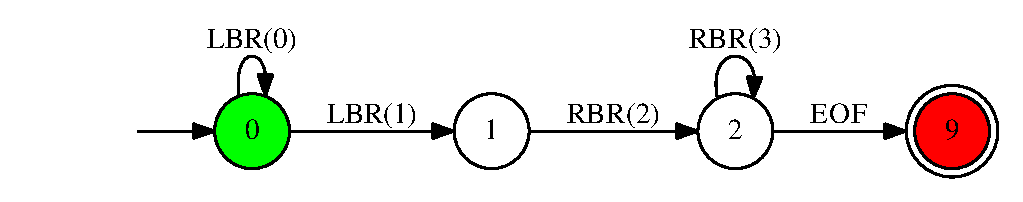
\includegraphics[scale=0.3]{dot/in3.eps}
   }  
   \hfill
    \subfloat[SPPF\label{resultSPPF}]{%
      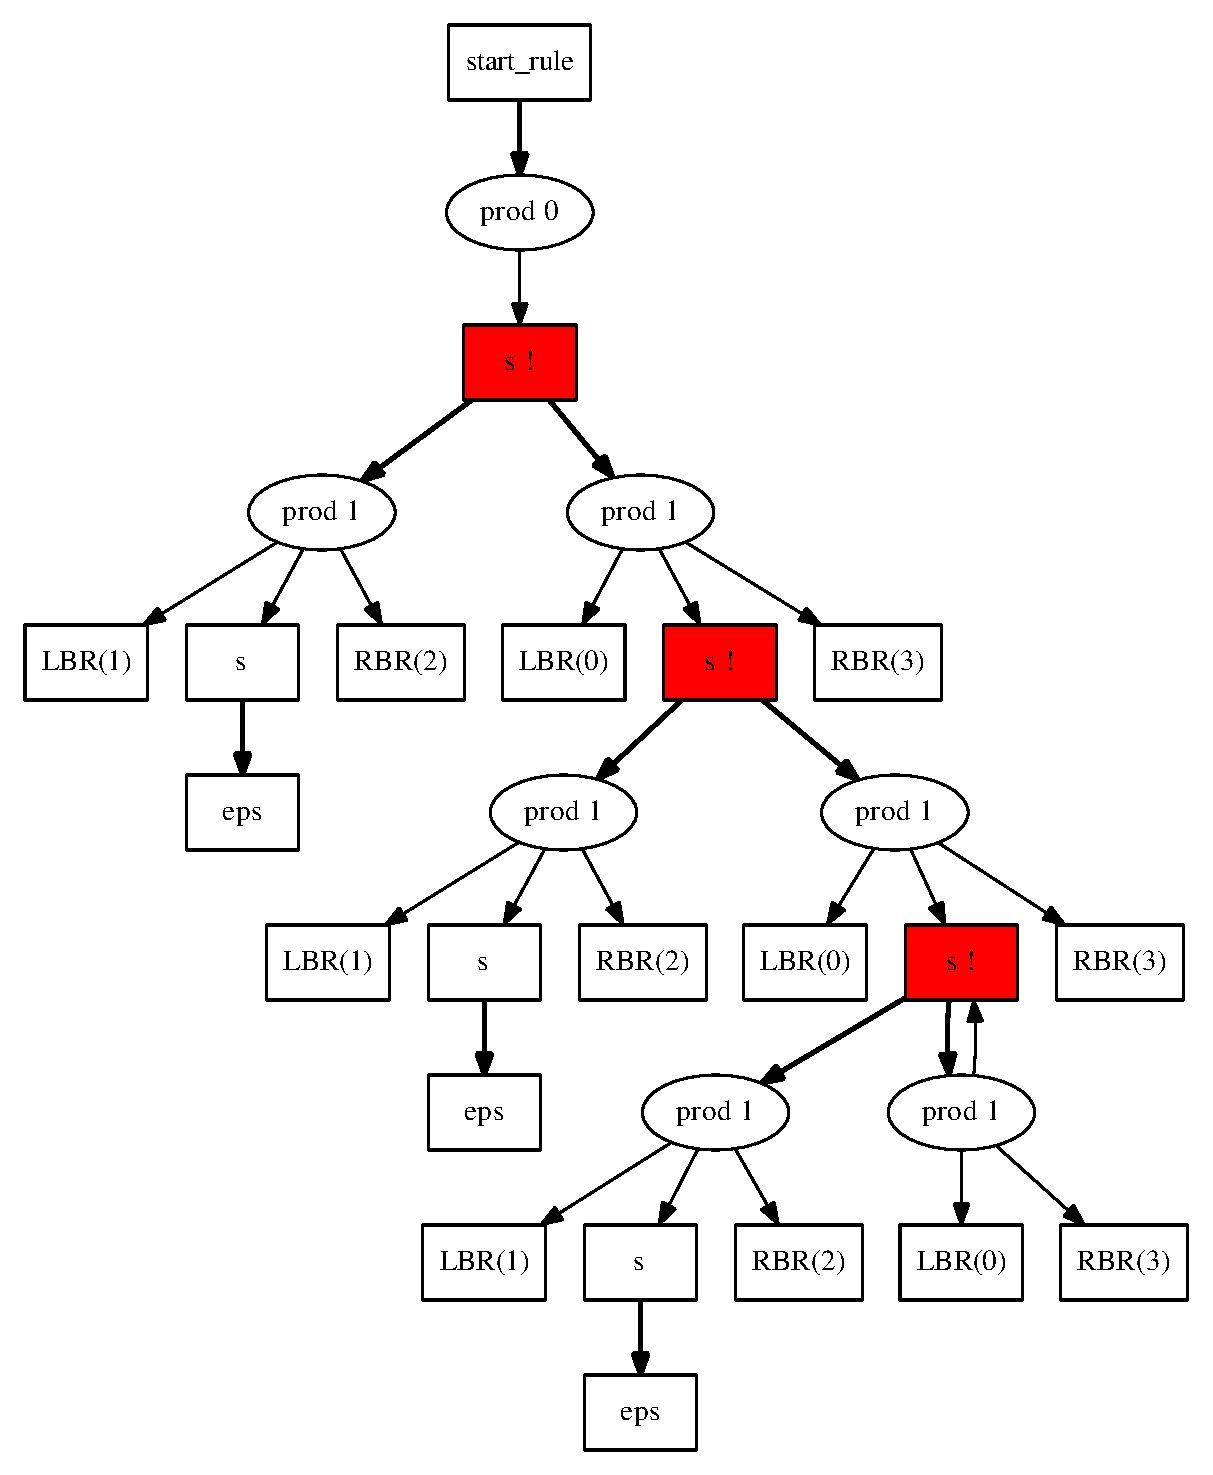
\includegraphics[scale=0.3]{dot/out3.eps}
    }
    \caption{Regular approximation and SPPF}
    \label{fig:SPPFforReg}
 \end{figure}

%\begin{figure}
%    \begin{center}
%        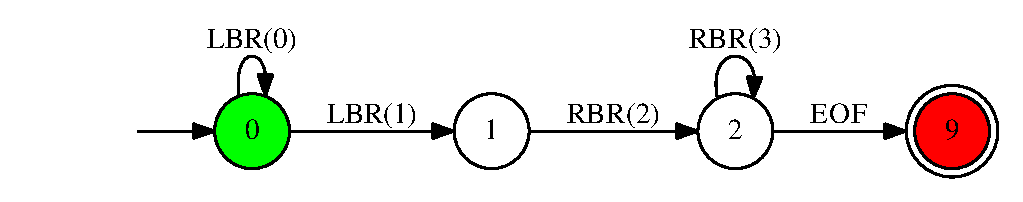
\includegraphics[scale=0.5]{dot/in3.eps}
%    \end{center}
%    \caption{$A_1$ -- input for our algorithm: regular approximation for string-embedded code after tokenization} 
%    \label{faApprox}
%\end{figure}

As it can be seen, some of the words from regular approximation do not belong to the reference language (for example, 
\verb|LBR LBR RBR|). The algorithm ignores such strings and constructs SPPF, which contains derivation trees 
for all recognized strings w.r.t. reference grammar.

%\begin{figure}
%    \begin{center}
%        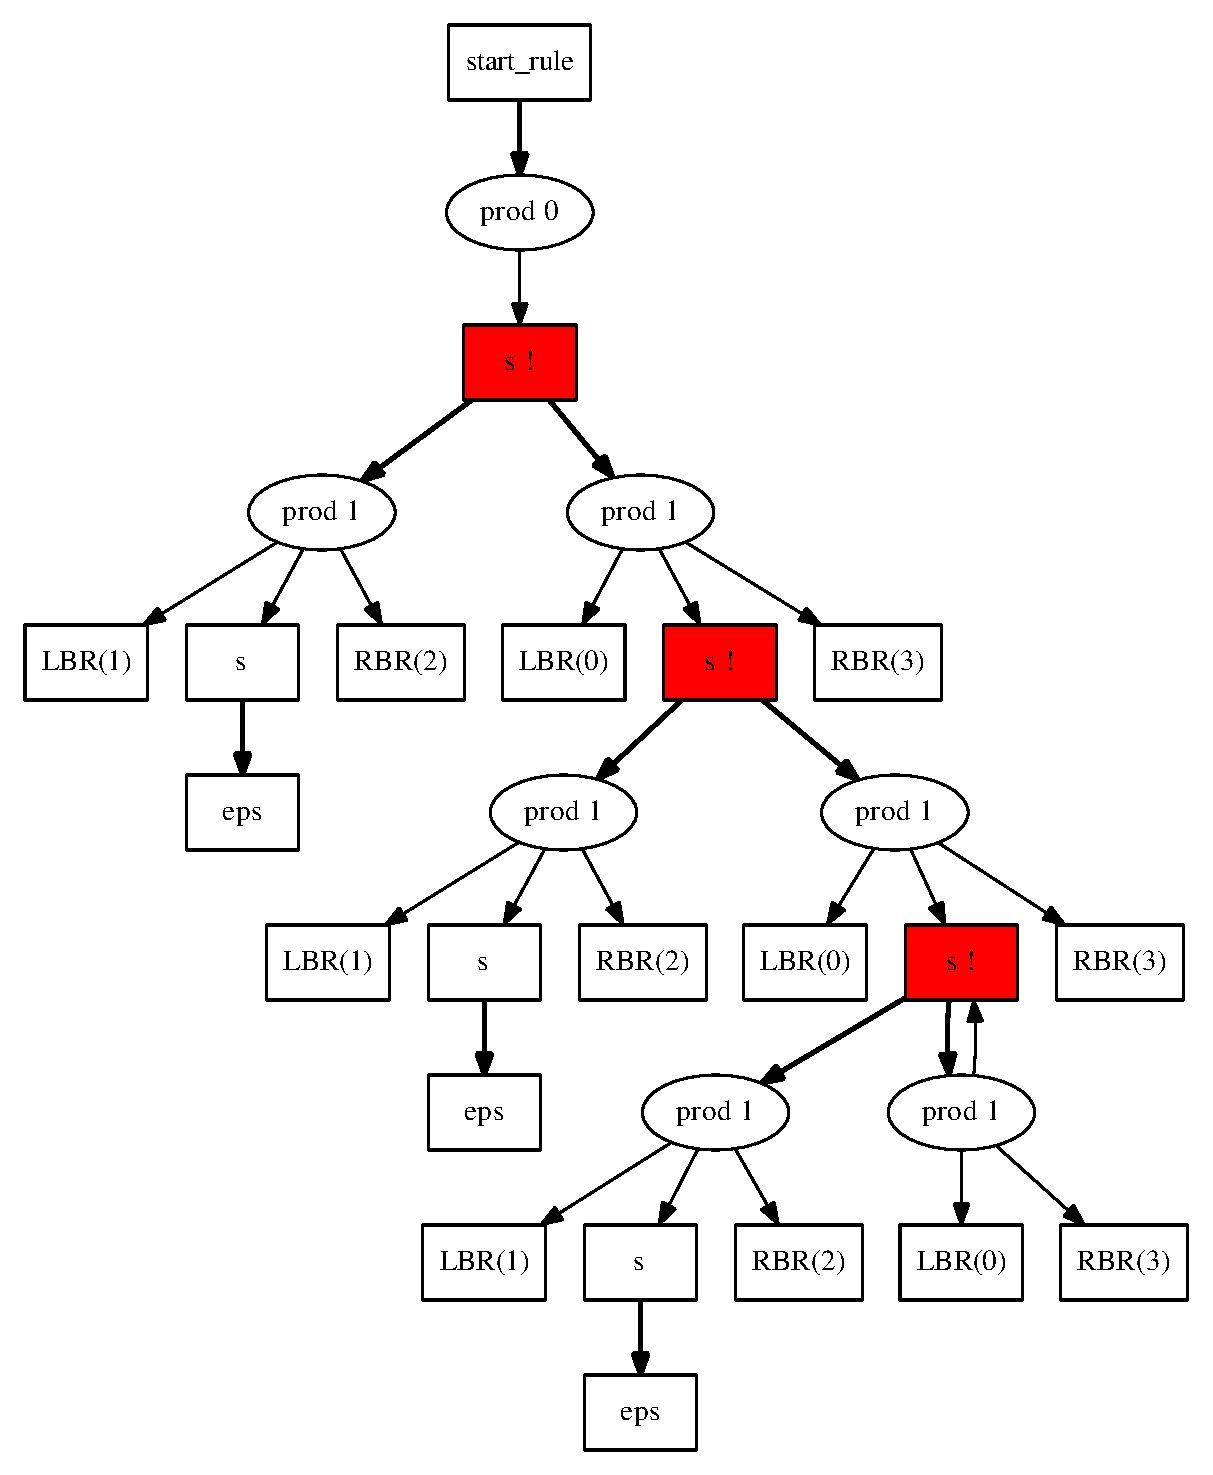
\includegraphics[scale=0.3]{dot/out3.eps}
%    \end{center}
%    \caption{SPPF for input FA presented in figure~\ref{faApprox}}
%    \label{resultSPPF}
%\end{figure}
\pagebreak
\section{\appendixname: RNGLR pseudocode}\label{RNGLRCode}

\begin{algorithm}[]
\begin{algorithmic}[1]
\caption{RNGLR algorithm}
\label{rnglr}
\Function{parse}{$grammar, input$}
  \State{$\mathcal{R} \gets \emptyset$} \Comment{Queue of tuples of GSS vertex, nonterminal, and reduction length}
  \State{$\mathcal{Q} \gets \emptyset$} \Comment{Collection of pairs of GSS vertex and parser state}
  \If{$input = \epsilon$}
    \If{$grammar$ accepts empty input} {report success}
    \Else { report failure}
    \EndIf
  \Else
    \State{\Call{addVertex}{$0, 0, startState$}}
    \ForAll{$i$ in $0..input.Length-1$}
      \State{\Call{reduce}{$i$}}
      \State{\Call{push}{$i$}}
    \EndFor
    \If{$i=input.Length-1$ and there is a vertex in the last level of GSS which state is accepting}
      \State{report success}
    \Else { report failure}
    \EndIf
  \EndIf
\EndFunction
\Function{reduce}{$i$}
  \While{$\mathcal{R}$ is not empty}
    \State{$(v, N, l) \gets \mathcal{R}.Dequeue()$}
    \State{find the set $\mathcal{X}$ of vertices reachable from $v$ along the path of length $(l-1)$}
    \State{or length $0$ if $l=0$}
    \ForAll{$v_{h} = (level_{h}, state_{h})$ in $\mathcal{X}$}
      \State{$state_{t} \gets$ calculate new state by $state_{h}$ and nonterminal $N$}
      \State{\Call{addEdge}{$i, v_{h}, v.level, state_{tail}, (l=0)$}}
    \EndFor
  \EndWhile
\EndFunction
\Function{push}{$i$}
  \State{$\mathcal{Q^{'}} \gets$ copy $\mathcal{Q}$}
  \While{$\mathcal{Q^{'}}$ is not empty}
    \State{$(v, state) \gets \mathcal{Q}.Dequeue()$}
    \State{\Call{addEdge}{$i, v, v.level + 1, state, false$}}
  \EndWhile
\EndFunction
\end{algorithmic}
\end{algorithm}

\begin{algorithm}[]
\begin{algorithmic}[1]
\caption{GSS construction}
\label{RNGLRMain}
\Function{addVertex}{$i, level, state$}
  \If{GSS does not contain vertex $v = (level, state)$}
    \State{add new vertex $v = (level, state)$ to GSS}
    \State{calculate the set of shifts by $v$ and the $input[i+1]$ and add them to $\mathcal{Q}$}
    \State{calculate the set of zero-reductions by $v$ and the $input[i+1]$ and}
    \State{add them to $\mathcal{R}$}
  \EndIf
  \State{\Return{$v$}}
\EndFunction
\Function{addEdge}{$i, v_{h}, level_{t}, state_{t}, isZeroReduction$}
  \State{$v_{t} \gets$ \Call{addVertex}{$i, level_{t}, state_{t}$}}
  \If{GSS does not contain edge from $v_{t}$ to $v_{h}$}
    \State{add new edge from $v_{t}$ to $v_{h}$ to GSS}
    \If{not $isZeroReduction$}
      \State{calculate the set of reductions by $v$ and the $input[i+1]$ and}
      \State{add them to $\mathcal{R}$}
    \EndIf
  \EndIf
\EndFunction
\end{algorithmic}
\end{algorithm}



\end{document}